\documentclass[a4paper,11pt]{article}
\usepackage[left=2.5cm, right=2.5cm, top=2cm, bottom=2.5cm]{geometry}
\usepackage{graphicx}
\usepackage{amssymb}
\usepackage{amsmath}
\usepackage{wrapfig}

\begin{document}
\title{\LARGE{\textbf{ECEN 202 Lab 4}\\Stepper Motor Driver}}
\author{Niels Clayton : 300437590\\ \textbf{Lab Partner: }Nickolai Wolfe}
\date{}
\maketitle

\section*{Introduction}
The task of this lab is to design and build the logic required to drive a stepper motor. A stepper motor is comprised of a stator and a rotor. The stator is a series of different coils that when a current is passed through then they will produce magnetic north and south poles. The rotor is comprised of a magnetically permeable material, that when the coils of the stator are on, will be attracted to the electromagnetic coils. To operate a stepper motor, these coils of the stator must be energized in the correct order. Because of this, we will be designing a counter that moves through the required states, in the required order to drive the motor. 
Our stepper motor driver must be able to:
\begin{enumerate}
\item Progress the motor both forwards and backwards
\item Stop the motor at any time, and then resume
\end{enumerate}

\section*{Design}

\begin{wrapfigure}{r}{8cm}
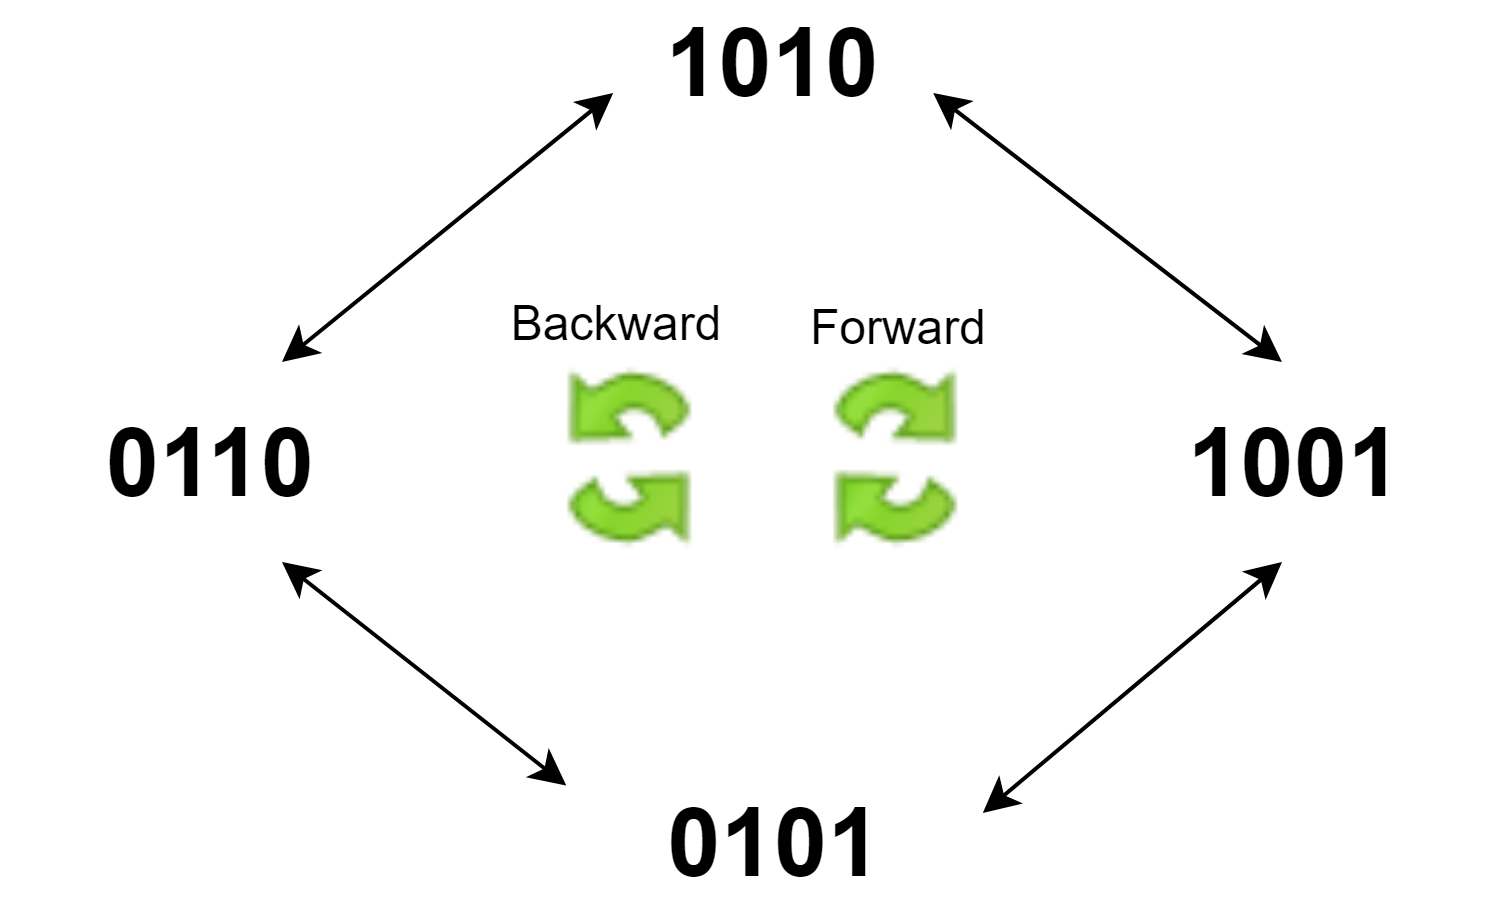
\includegraphics[width = 7cm]{States.png}
\caption{States of the counter}
\end{wrapfigure}

The states that our counter must cycle though are shown in figure 1. While cycling, progressing clockwise around the diagram will rotate the motor in the forward direction, and progressing anti-clockwise will rotate the motor backwards. In order to simplify the logic for the counter, it can be observed that bits 1 \& 2 as well as bits 3 \& 4 are inverse of each other. Because of this, each number in the sequence can be thought of as  $Q_{1} \overline{Q_{1}} Q_{3} \overline{Q_{3}}$, decreasing the number of outputs we will need to work with since since a single flip-flop can provide both $Q$ and $\overline{Q}$. We will also be able to simplify our circuits by using D-flip-flips rather than JK's, as D's will only require the required output to be placed on the input of the flip-flop.\\
\linebreak
Using this state diagram we are able to draw a table of inputs $E$ (enable), \& $D$ (direction), alongside our current outputs  $Q_{1}$ \& $Q_{3}$. Then by comparing the desired next state of our outputs to their current state, we can determine the input into the D-flip-flop required to provide the next state. This Logic table can be seen in figure 2.\\
\newpage
\begin{figure}[h]
\centering
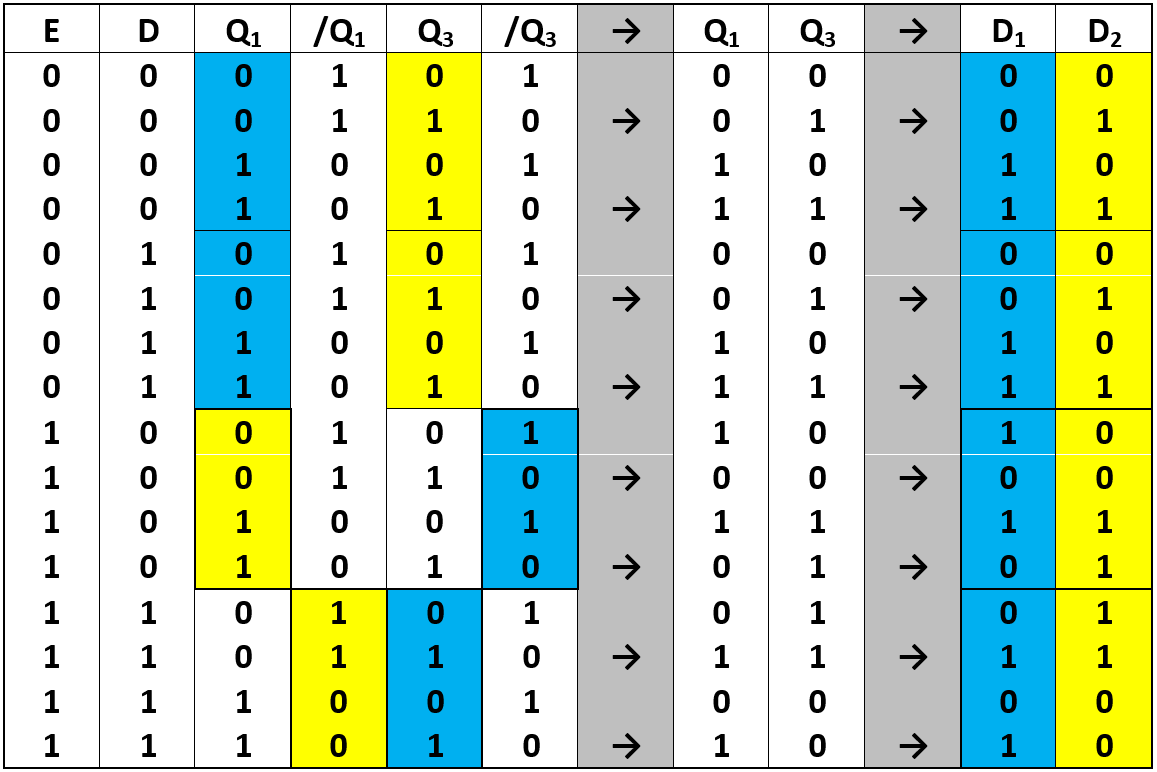
\includegraphics[width=\linewidth]{state_table.png}
\caption{current and required states of the counter}
\end{figure}
By looking at this table, we are able to see that when the enable $E$ input is low, whatever value is currently on $Q_{1}$ \& $Q_{3}$ must remain the same. This means that onto the input of the D-flip-flop's $D_{1}$ \& $D_{2}$ we can directly connect their outputs of $Q_{1}$ \& $Q_{3}$.\\
Once the enable input is high, we can see from the table that the input's required into each flip-flop are current outputs of the flip flops. From this we can deduce that if the enable and direction ($E \& D$) are high, then $D_{1} = Q_{3}$ \& $D_{2} = \overline{Q_{1}}$. And if enable is high and direction is low ($E \& \overline{D}$) then $D_{1} = \overline{Q_{3}}$ \& $D_{2} = Q_{1}$.
\\[5pt]

From here we can take the enable and direction inputs, and use them as the selection lines on two 4:1 MUX chips. These MUX's will then take the D-flip-flop outputs of $Q_{1}, \overline{Q_{1}}, Q_{3}, \overline{Q_{3}}$, and use them as the inputs of the MUX's as shown in figure 3. This sequence will then be stepped along using a 1Hz clock signal that will be generated by a generic 555 timer chip.
\begin{figure}[h]
\centering
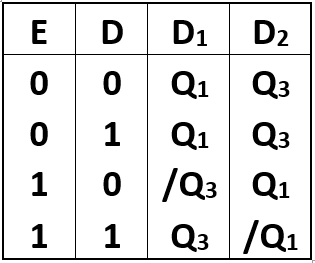
\includegraphics[width = 5cm]{mux_table.png}
\caption{States of the counter}
\end{figure}
\newpage
\begin{figure}[h]
\centering
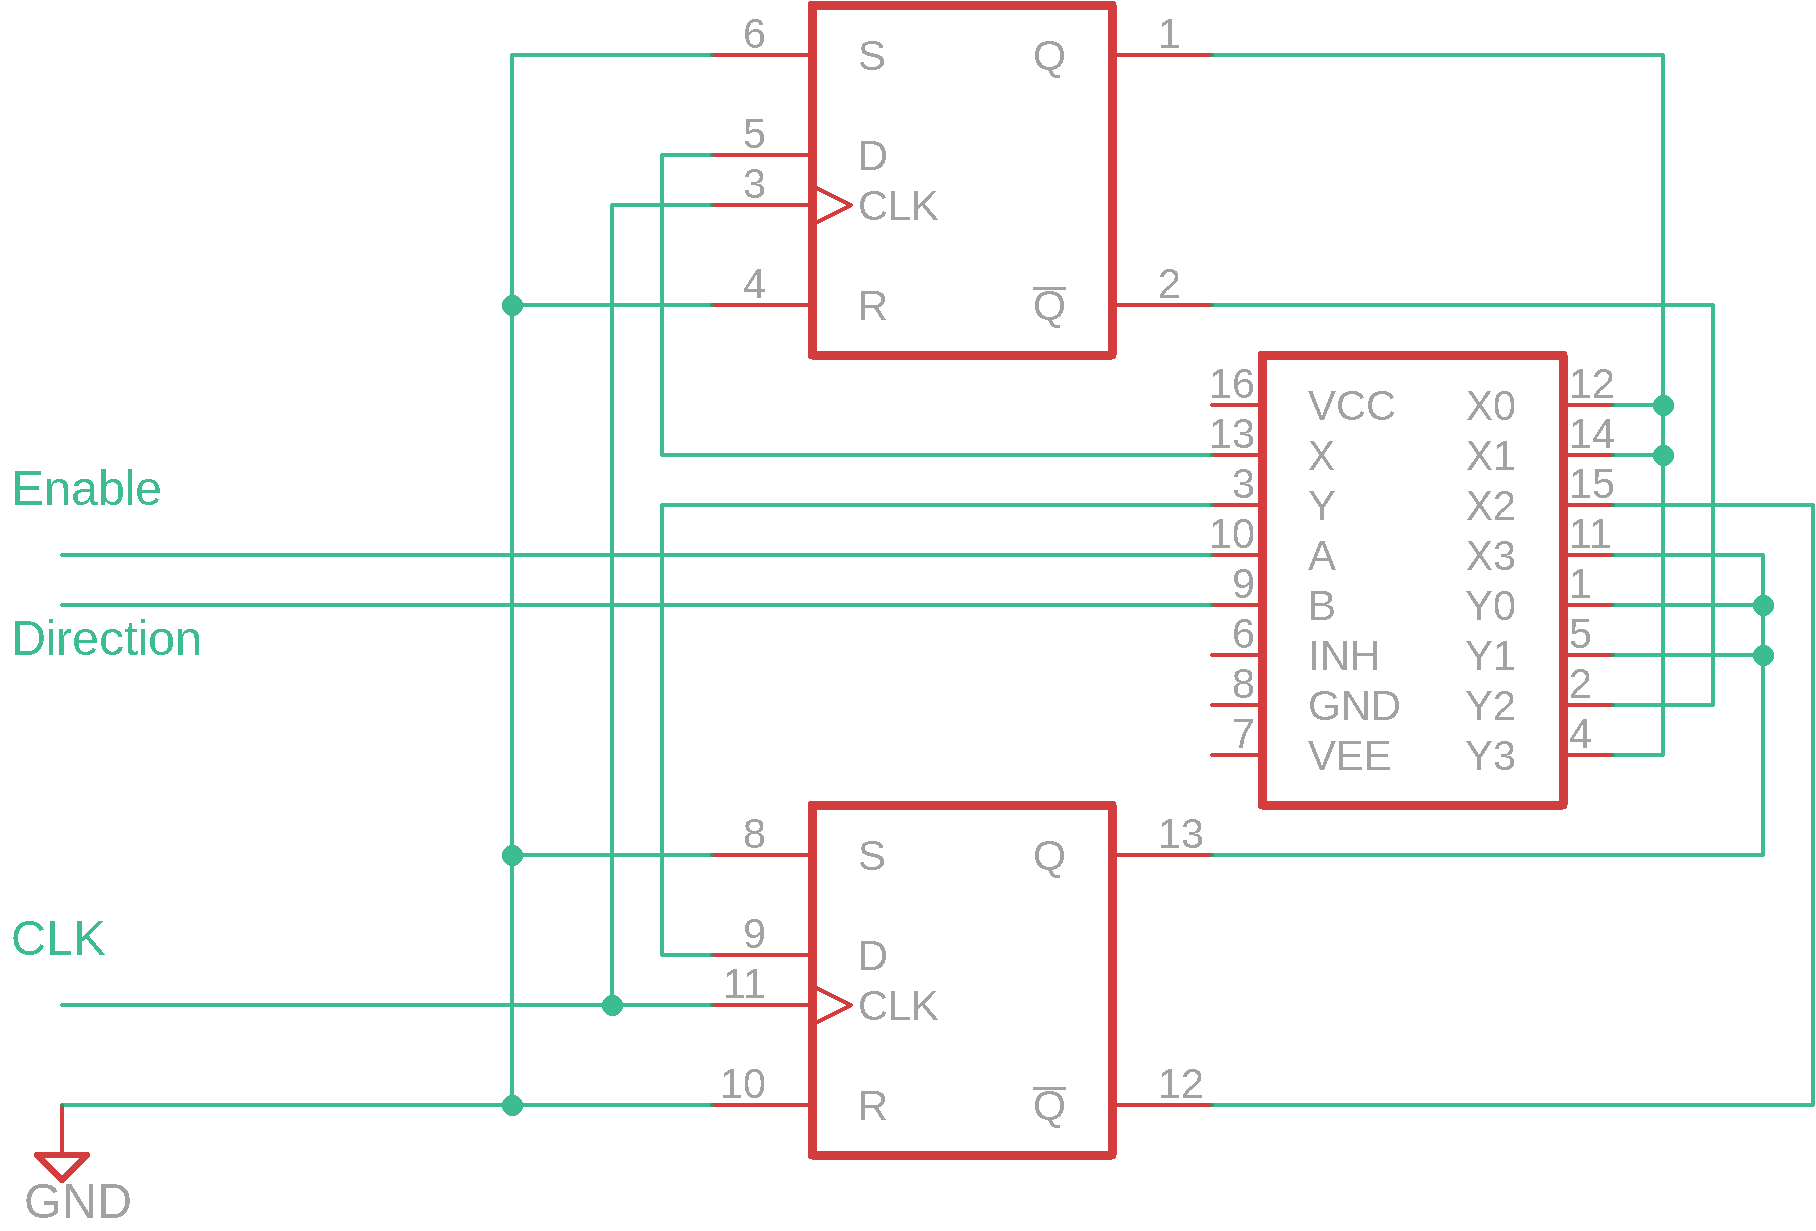
\includegraphics[width = \linewidth]{circuit.png}
\caption{Design of main counter circuit}
\end{figure}
\begin{figure}[h]
\centering
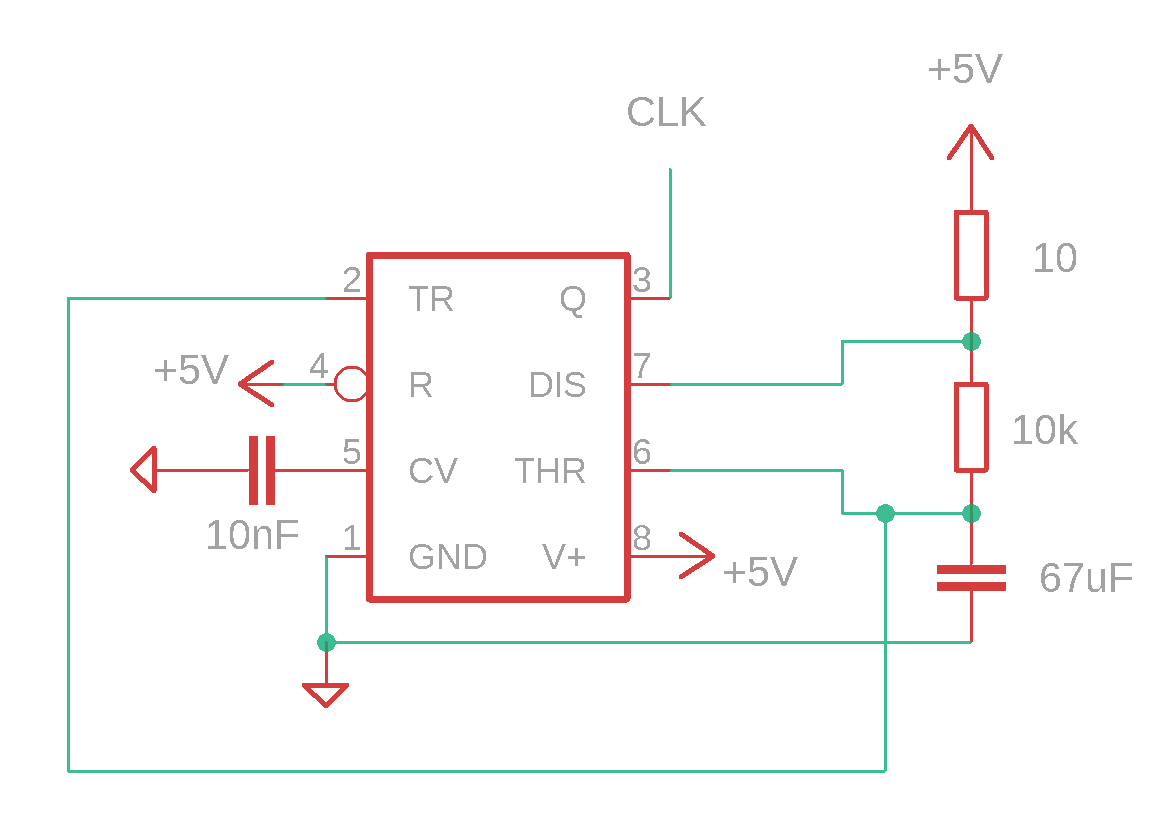
\includegraphics[width = 8.5cm]{CLK_timer.png}
\caption{1Hz frequency 555 timer curcuit}
\end{figure}
Figure 4 is a sketch up of the circuit that was build. This circuit will be comprised of two chips, one 74HCT374 dual D-flip-flop IC, and one 74HCT153 dual 4:1 multiplexer. Figure 5 is the sketch up of the 1Hz generating 555 timer circuit. This one Hz square wave signal will be used as the clock signal for the counting circuit.
\newpage
\begin{figure}[h]
\centering
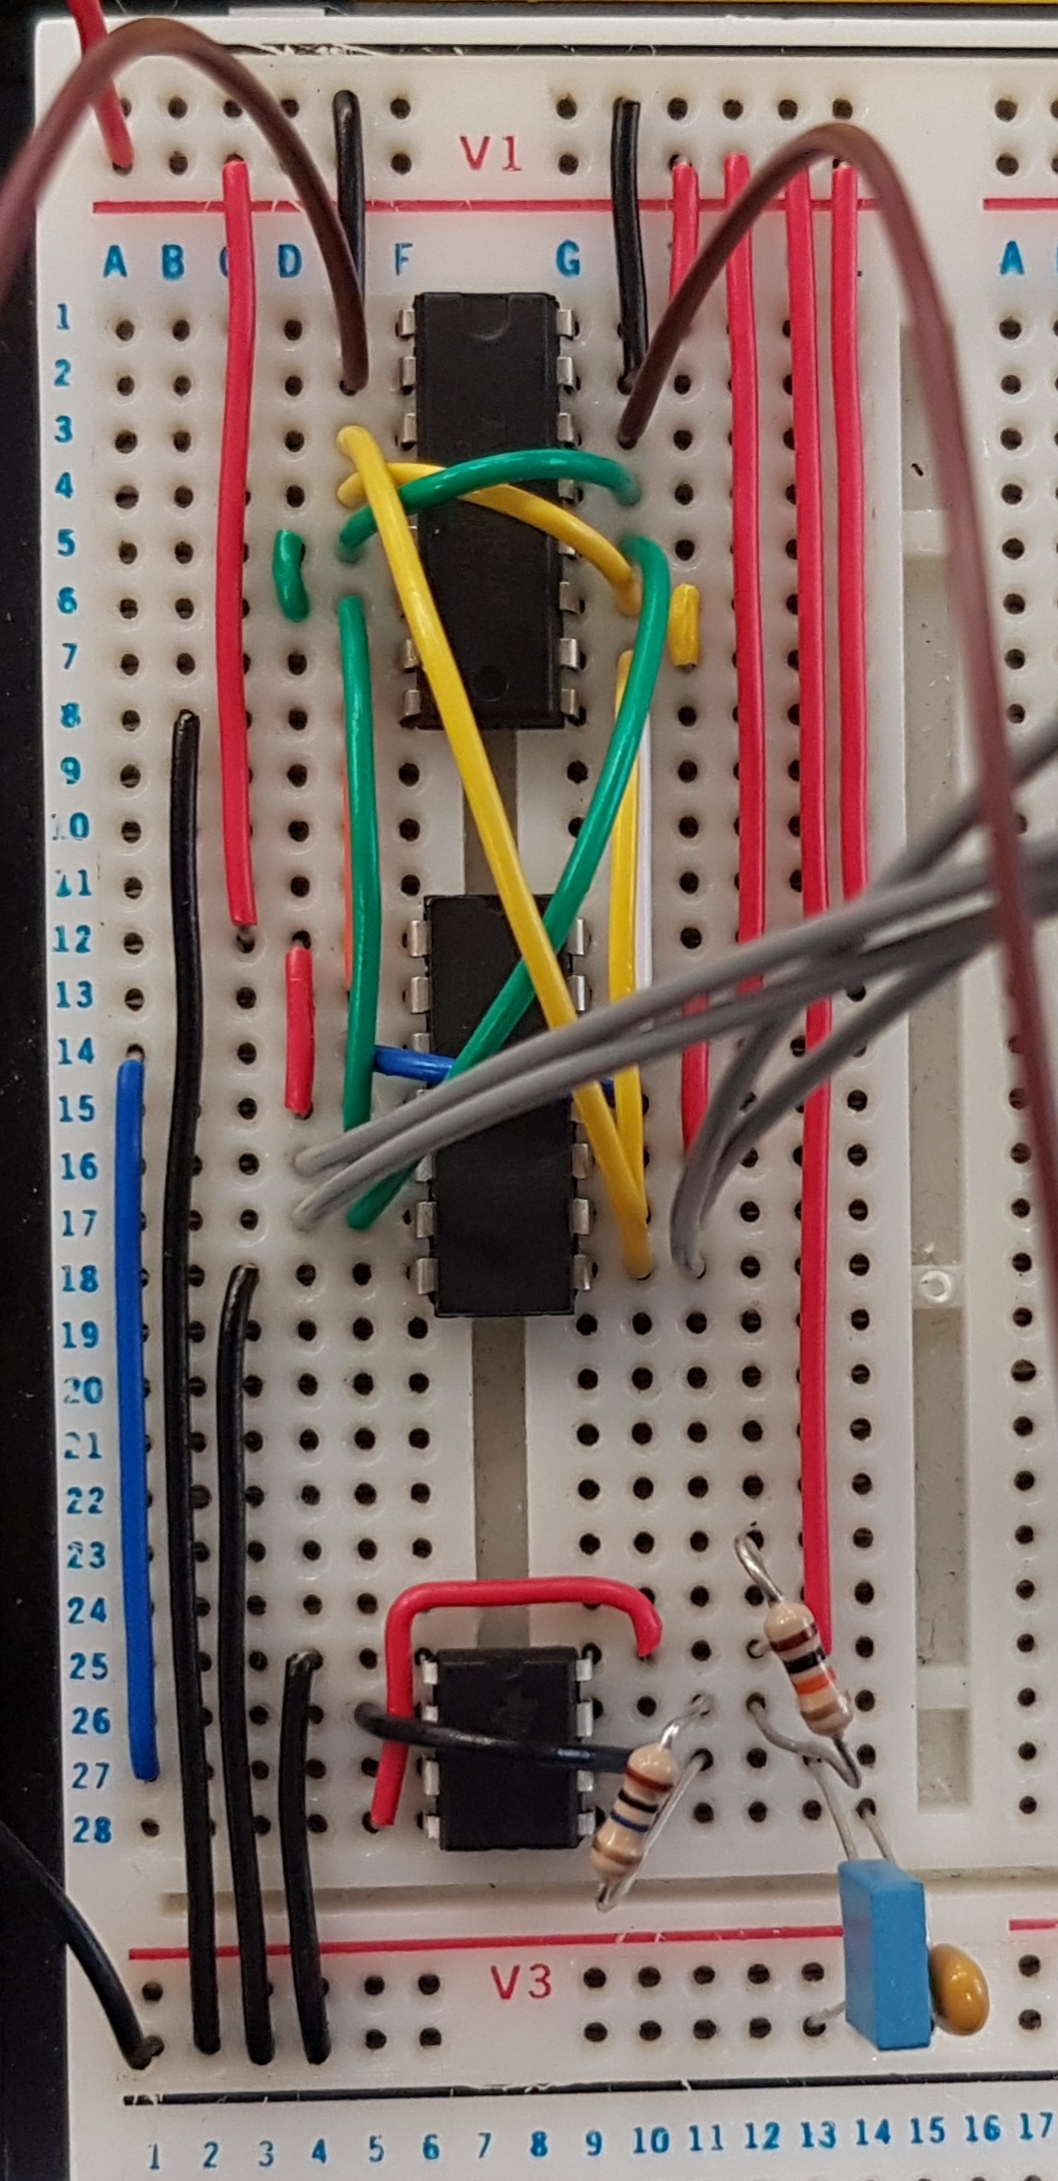
\includegraphics[width = 8cm]{20190410_152117(1).jpg}
\caption{Test build of circuit on breadboard}
\end{figure}
When testing the circuit, it worked just as expected, and correctly allowed for operation of the stepper motor, and also allowing for changes of direction, and stopping the motor.

\section*{Conclusion}
After the simplification of the states of the counter, replicating it became a relatively simplistic task, and produced a very minimalistic circuit that achieves the wanted results. This simplification process could again be simplified if you were to recognise the pattern within the original sequence. Also another way to achieve a similar result to what we have made would be to use either a single H-bridge chip, or a small micro-controller such as an ATtiny85, which would both be single chip solutions. 

\end{document}
